\section{Introduction}

\begin{figure}[!ht]
    \centering
    \subfigure[RWKV-7-4K 2.9B]{%
        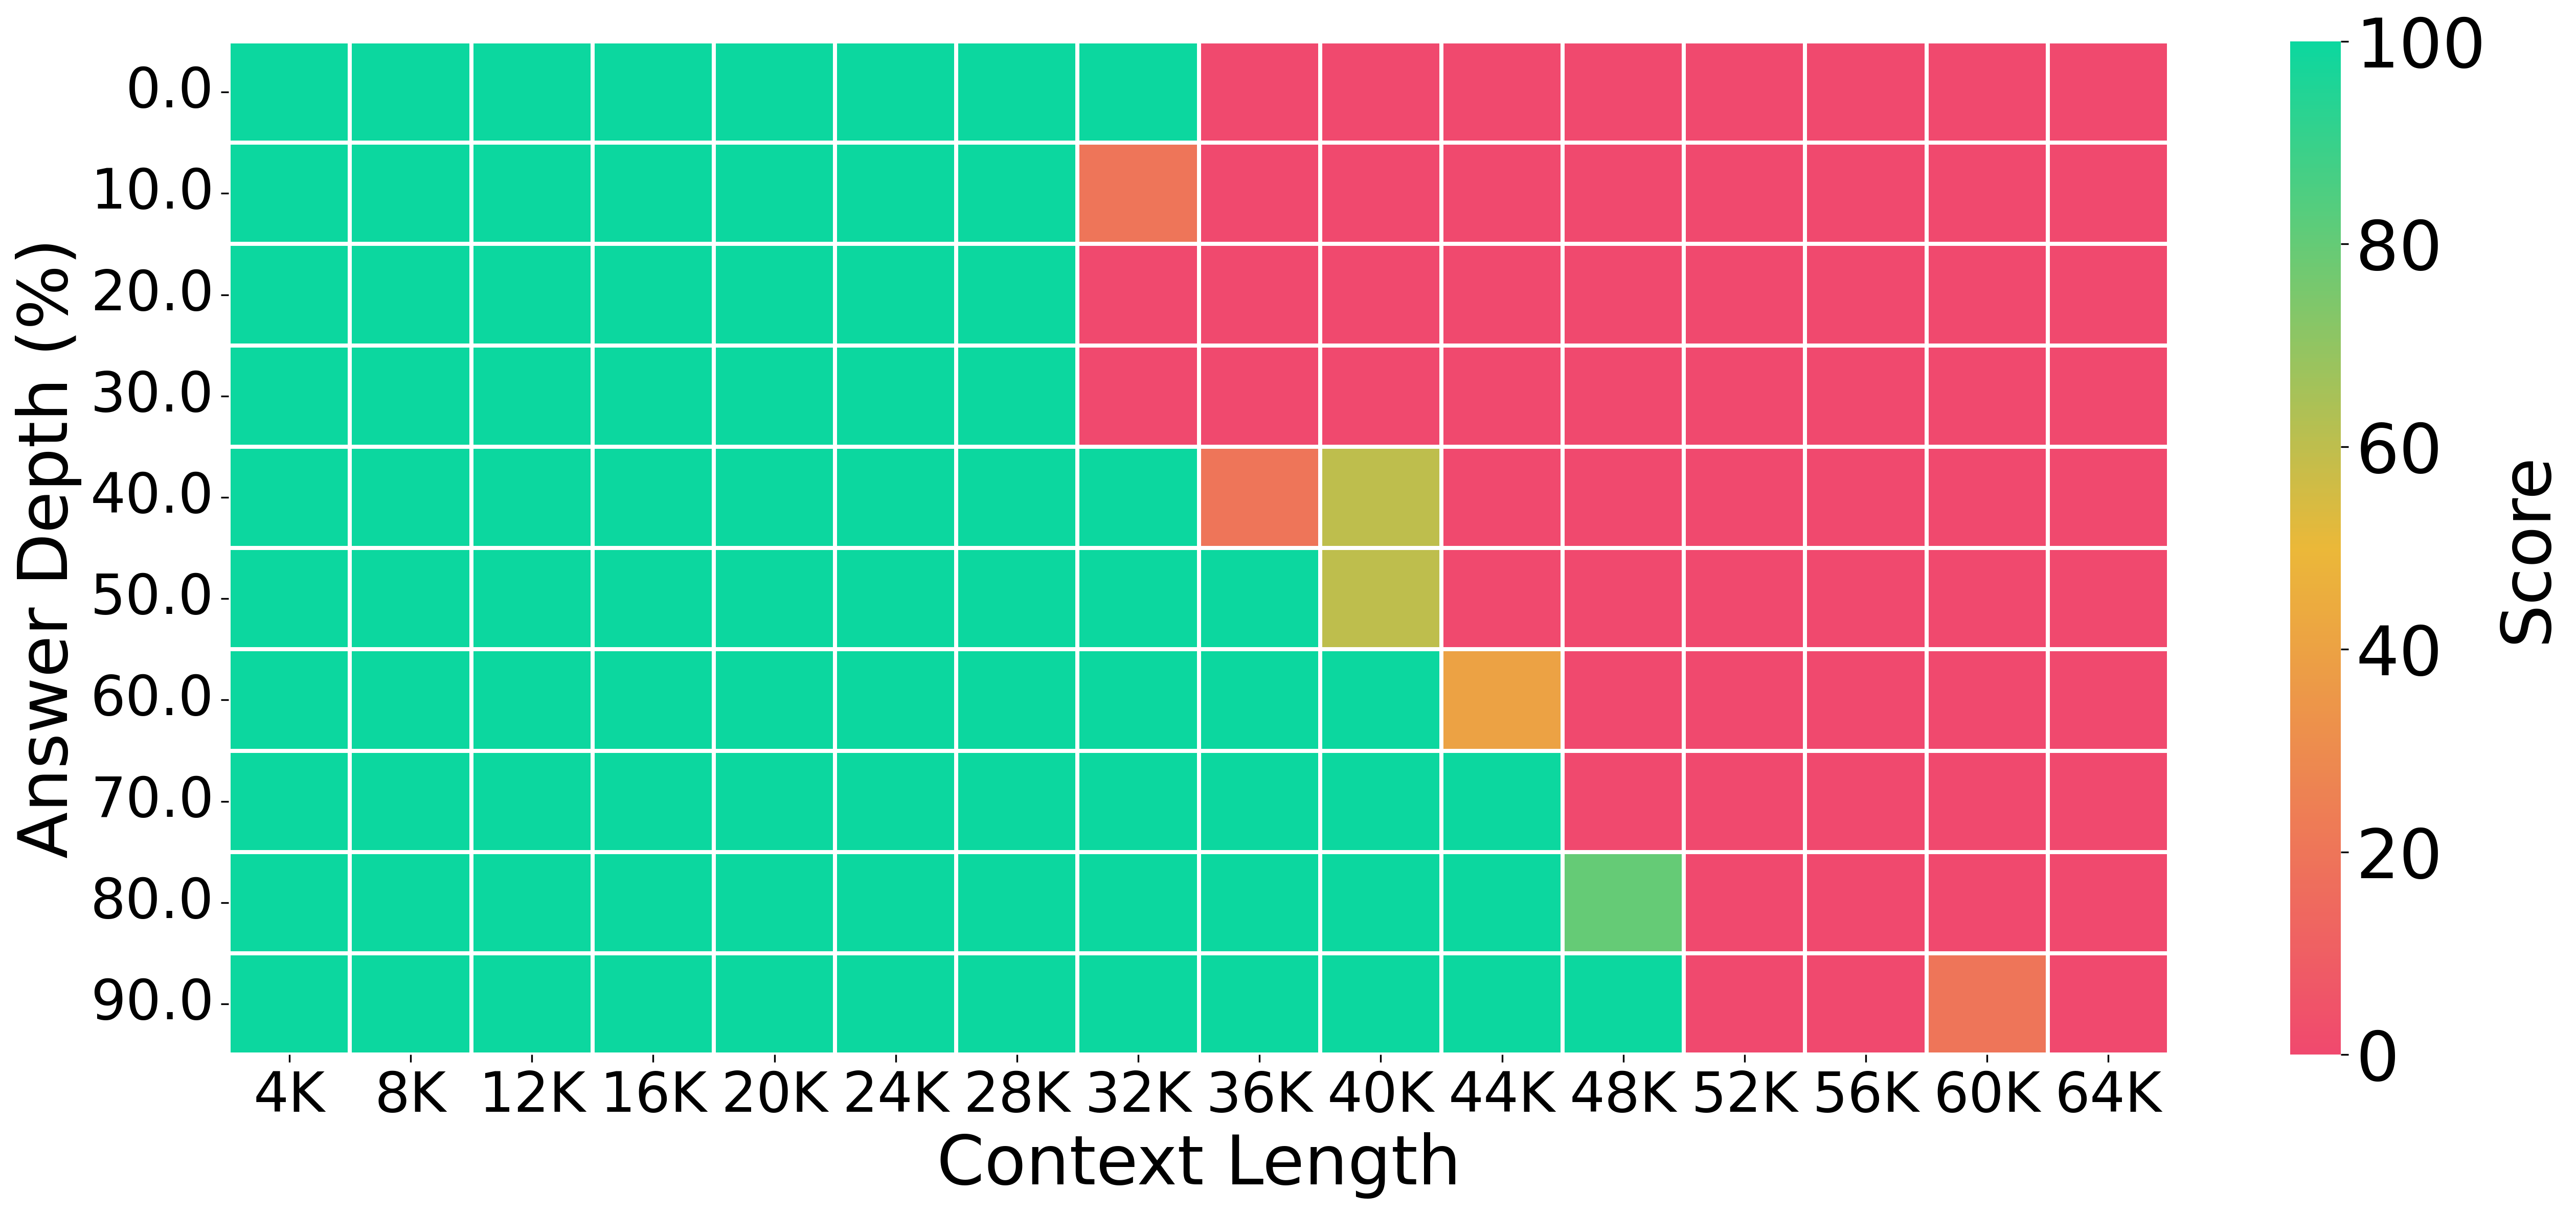
\includegraphics[width=\linewidth]{figures/RWKV-x070-World-2.9B-v3-20250211-ctx4096_heatmap_64000.png}
        \label{fig:passkey_rwkv7-4k}
    }
    \subfigure[RWKV-7-128K 2.9B]{%
        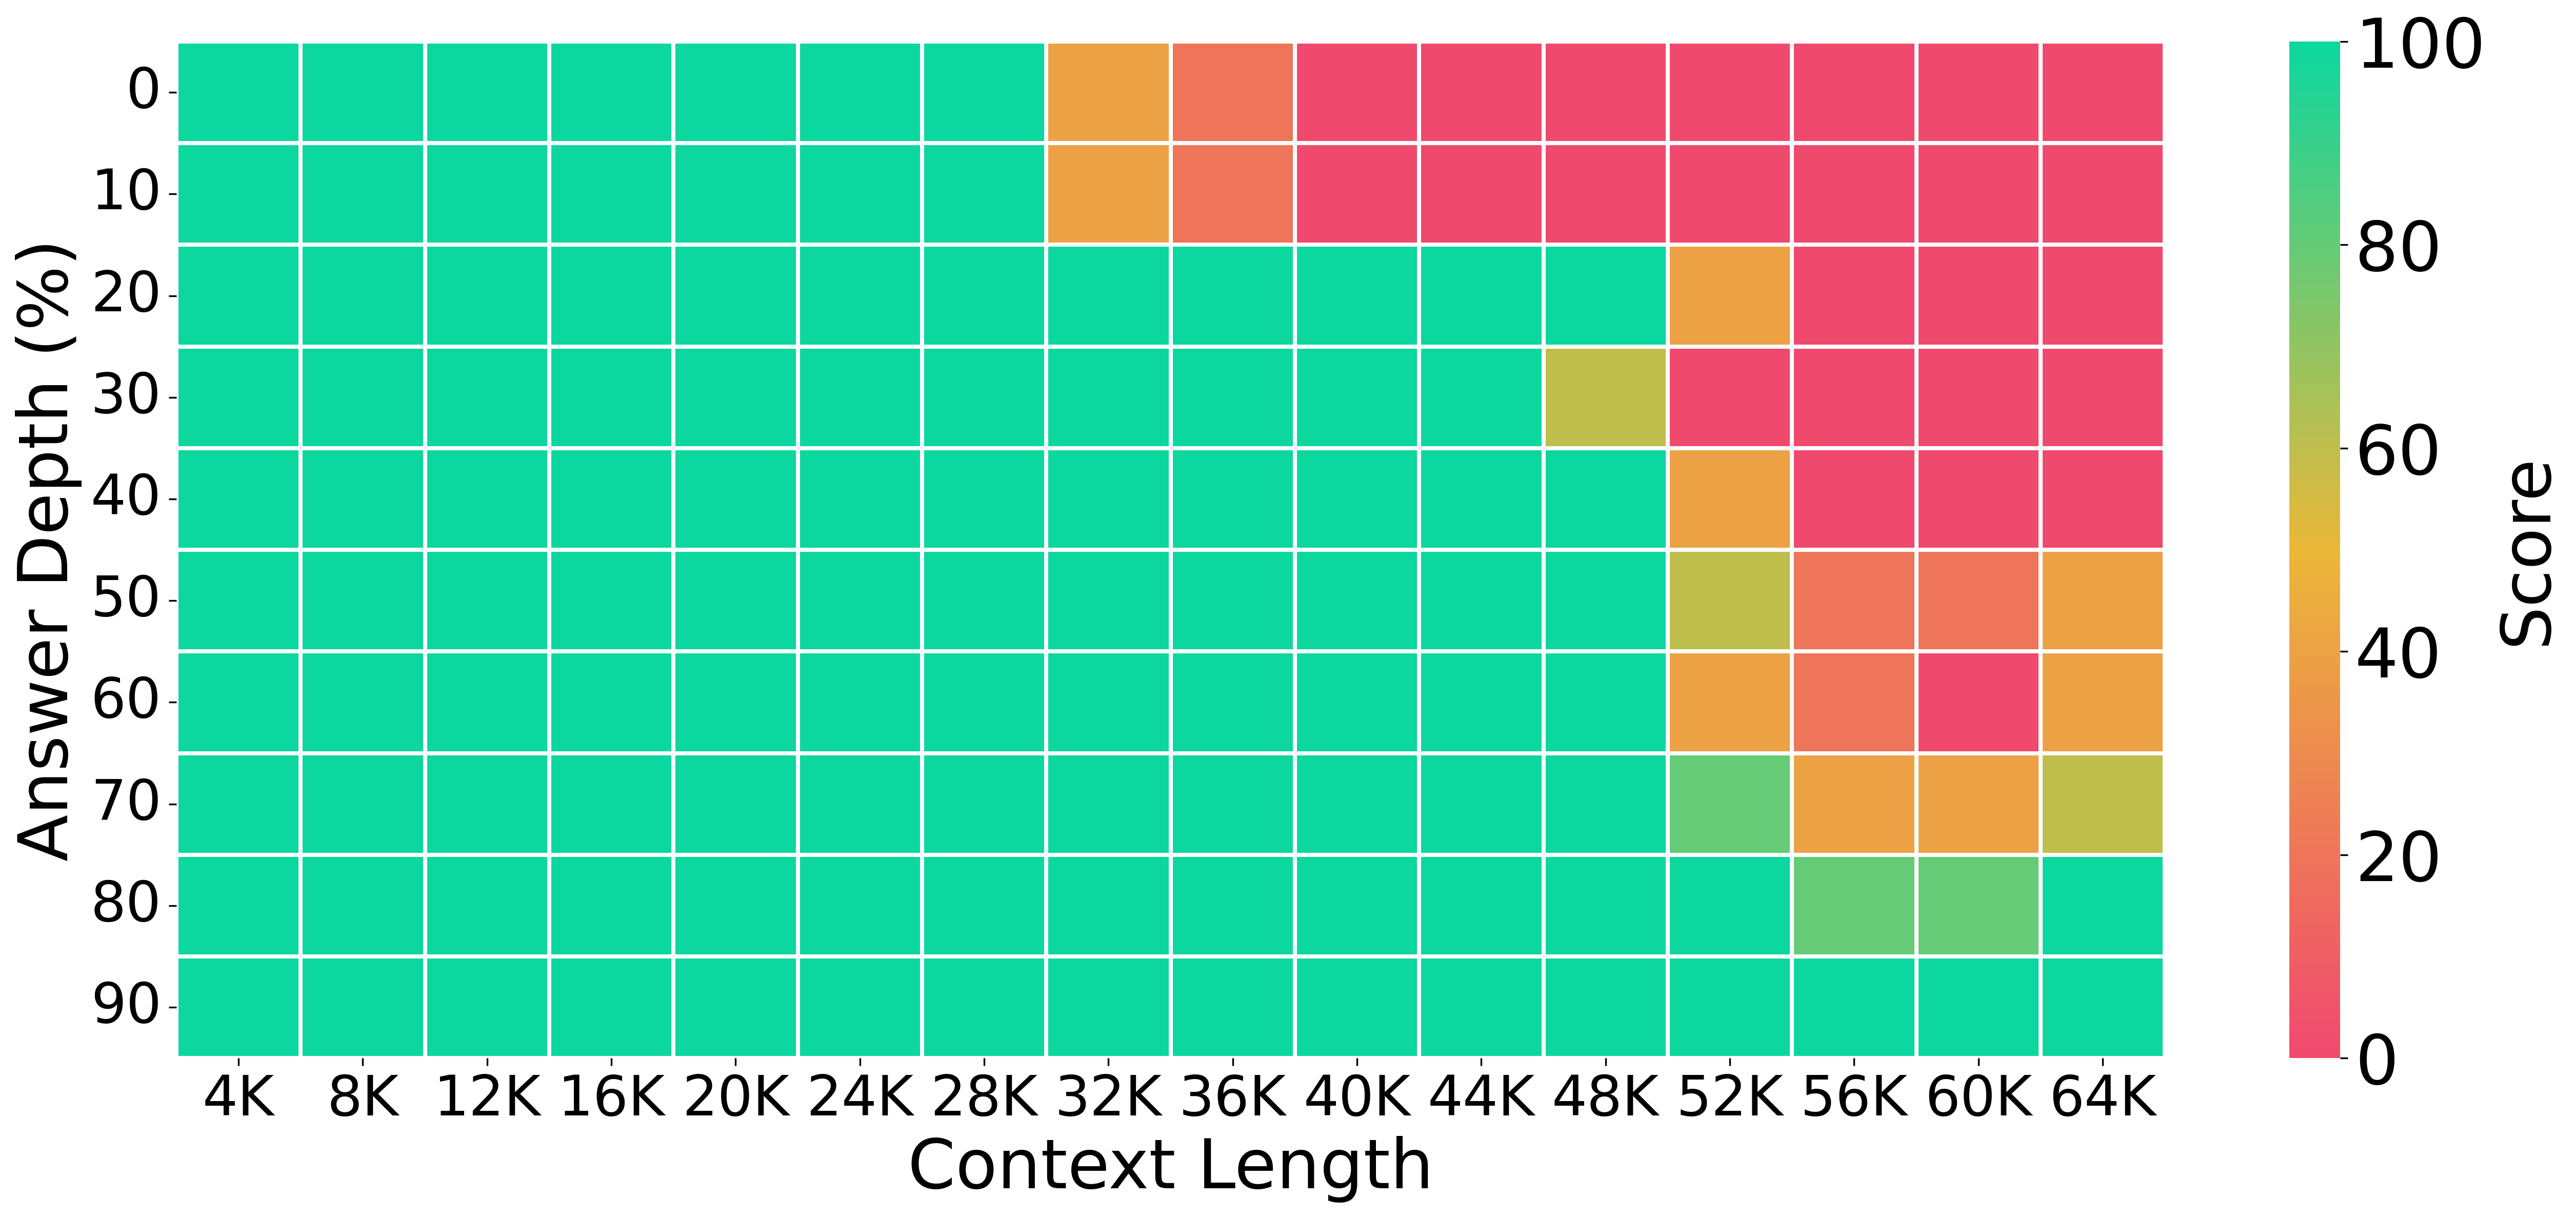
\includegraphics[width=\linewidth]{figures/RWKV-x070-World-2.9B-v3-ctx128K_heatmap_64000.png}
        \label{fig:passkey_rwkv7-128k}
    }
    \subfigure[RWKV-X-64K 3.6B]{%
        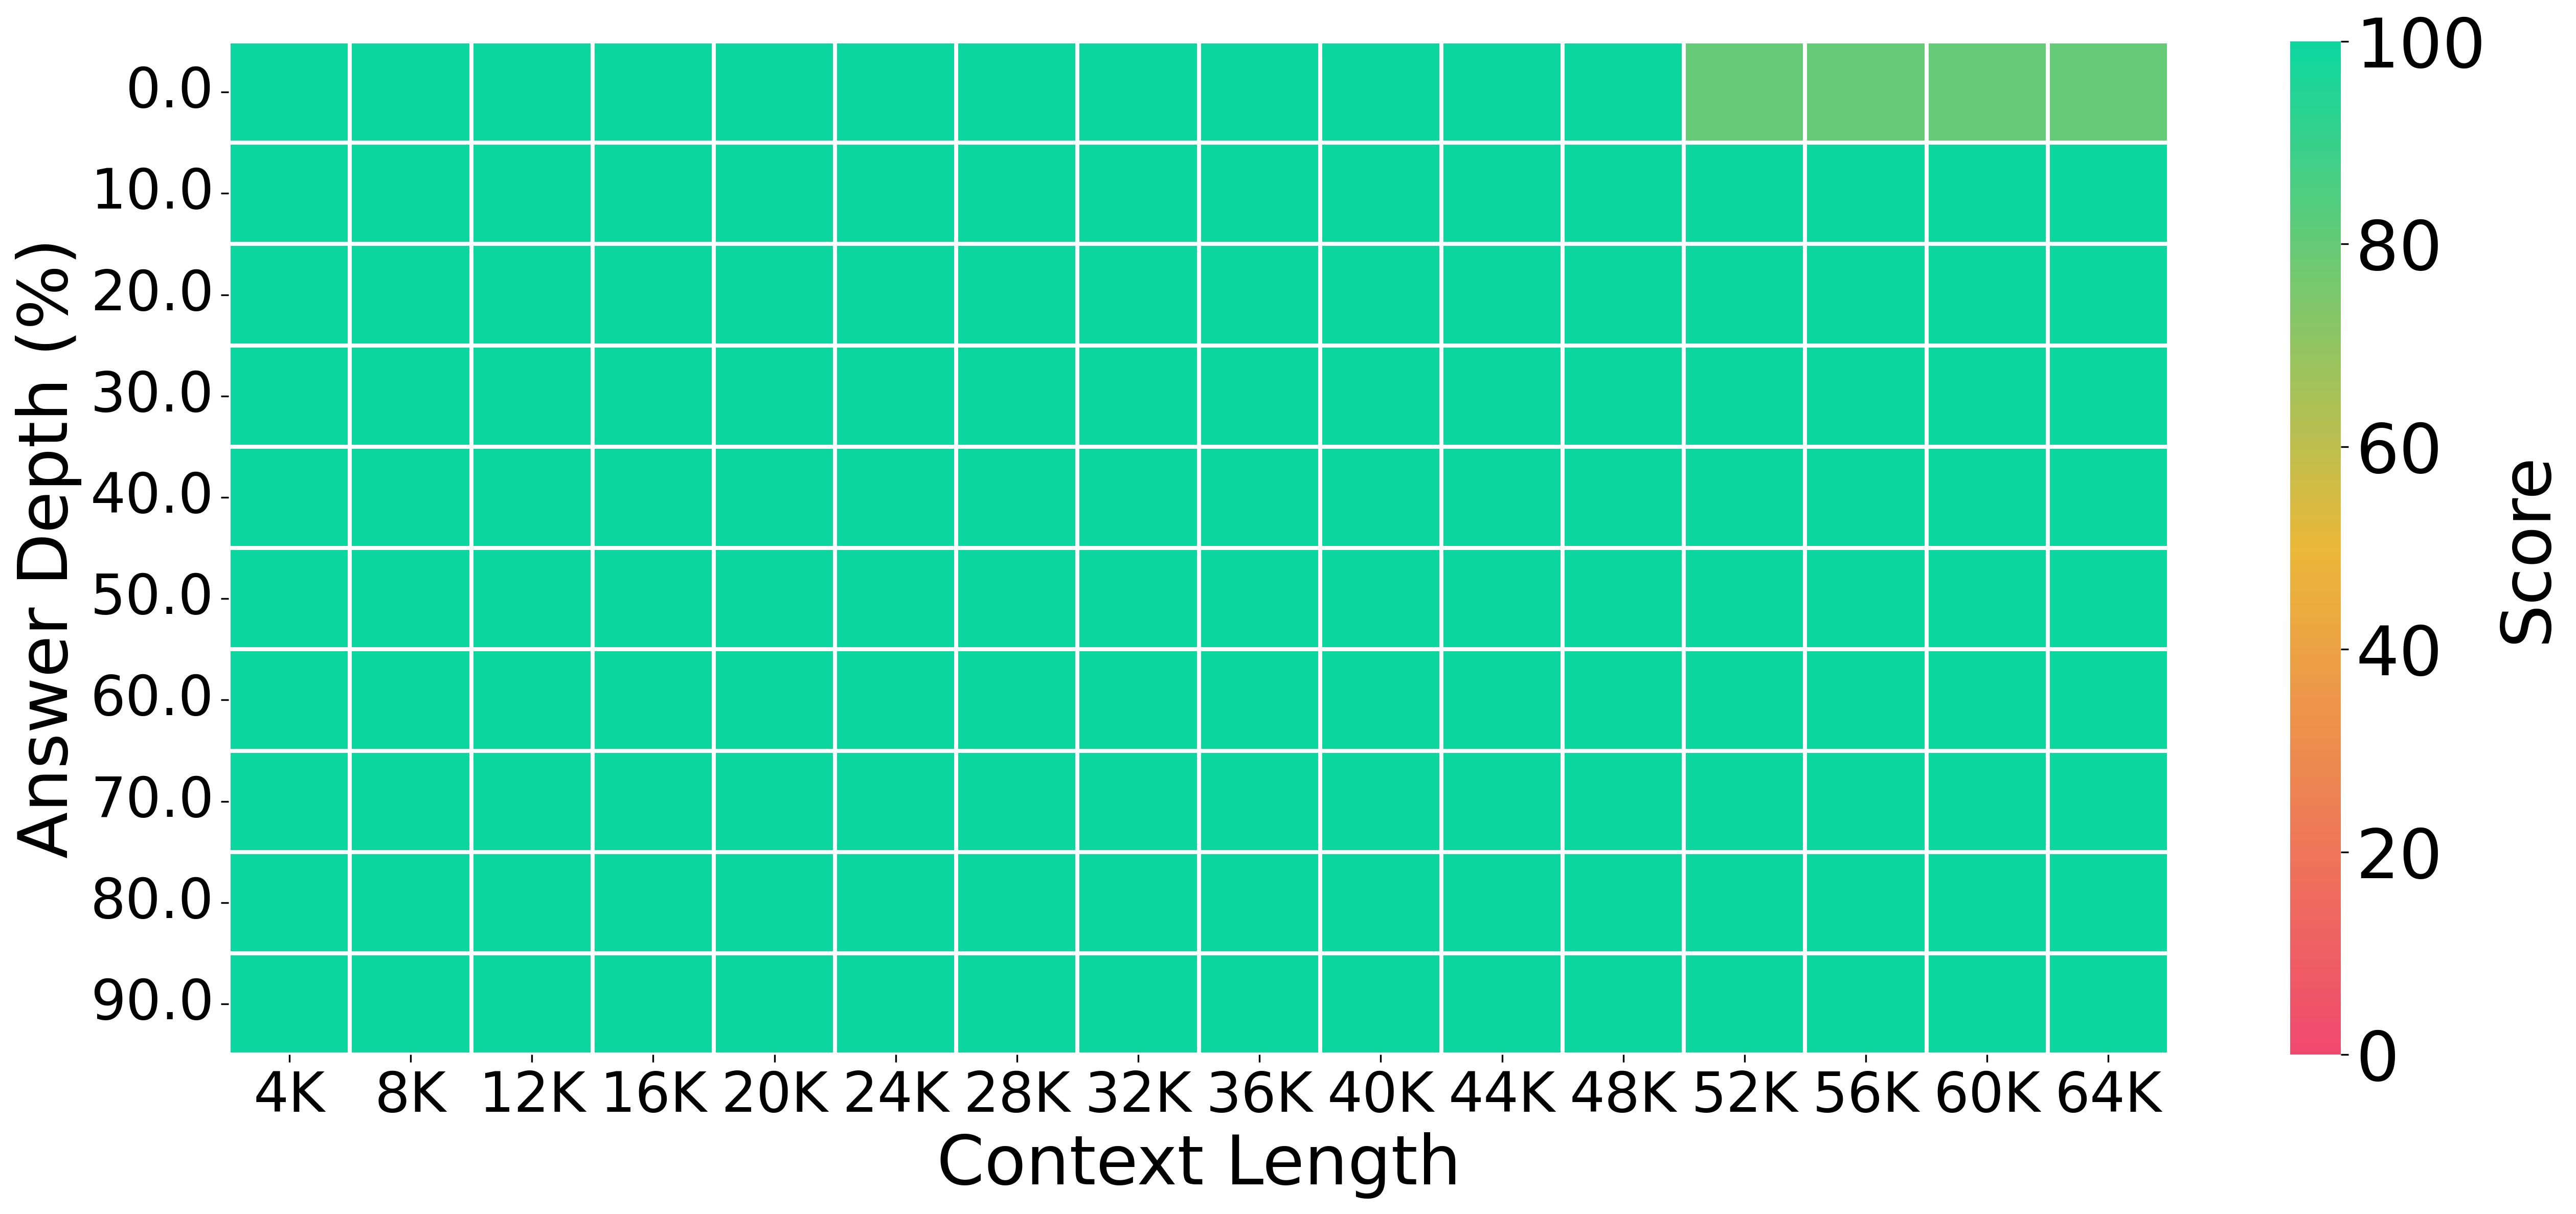
\includegraphics[width=\linewidth]{figures/RWKV-X-3.6B-64k-Base_heatmap_64000.png}
        \label{fig:passkey_rwkvx-64k}
    }
    \caption{Passkey retrieval performance of RWKV-X models on documents up to 64K tokens. Results are shown for: (a) RWKV-7 pretrained with a 4K context length; (b) RWKV-7 after continual pretraining with a 128K context length; and (c) RWKV-X trained with continual pretraining on a 64K context length.}
    \label{fig:passkey}
\end{figure}

Transformers have become the foundation of modern large language models (LLMs), but their quadratic complexity in sequence length poses significant limitations when scaling to long-context inputs. 
To address this, a range of alternatives has emerged, including Linear Attention models~\cite{katharopoulos2020transformers}, State Space Models (SSMs) such as Mamba~\cite{gu2023mamba}, and Linear RNNs such as DeltaNet~\cite{yang2024parallelizing} and RWKV~\cite{peng2023rwkv, peng2025rwkv7gooseexpressivedynamic, peng2024eagle}.
Linear RNN-based architectures demonstrate competitive performance compared to Transformers under similar model sizes and training budgets, while significantly reducing inference costs.

However, despite their efficiency, current linear architectures still struggle with long-context understanding. 
As shown in Figure~\ref{fig:passkey_rwkv7-4k}, RWKV-7 (2.9B) achieves high accuracy on passkey retrieval up to 28K tokens, but performance rapidly degrades beyond that point. While continual pretraining with 128K-length data offers modest improvements (Figure~\ref{fig:passkey_rwkv7-128k}), long-context limitations remain. 
This limitation is not unique to RWKV; similar observations have been reported in other architectures such as Mamba~\cite{chen2024stuffed}, highlighting a broader challenge for this class of models~\cite{arora2023zoologymeasuringimprovingrecall}.

A promising approach to mitigating this limitation is the use of hybrid models that combine full attention with linear attention layers, as demonstrated in systems such as Jamba~\cite{Lieber2024JambaAH} and Zamba~\cite{glorioso2024zambacompact7bssm}. 
While these architectures improve long-context performance to some extent, their reliance on full attention layers preserves quadratic complexity, resulting in memory bottlenecks during inference over very long sequences.

In this work, we propose RWKV-X, a novel hybrid model with linear complexity that combines the strengths of RWKV for modeling short-range dependencies and sparse attention for capturing long-range context.
As shown in Figure~\ref{fig:passkey_rwkvx-64k}, RWKV-X is continually pretrained on 64K-token sequences and achieves near-perfect accuracy on the 64K passkey retrieval benchmark.

Experimental results demonstrate that RWKV-X substantially improves performance on long-context benchmarks while maintaining competitive accuracy on short-context tasks. In terms of system efficiency, RWKV-X achieves linear-time complexity ($O(N)$) during training and constant-time complexity ($O(1)$) during inference decoding. These results highlight RWKV-X as a highly effective and scalable backbone for general-purpose language modeling across both short and long contexts.

Our main contributions are as follows:
\begin{itemize}
    \item We propose RWKV-X, a novel hybrid model that achieves linear complexity in both training and inference, while effectively modeling long-range dependencies.
    \item We develop a sparse attention mechanism with linear complexity, which integrates seamlessly with the RWKV architecture to enhance long-context modeling.
    \item RWKV-X outperforms baseline models on long-context benchmarks, while maintaining strong performance on short-context tasks.
    \item RWKV-X enables ultra-long-range decoding with constant inference speed and memory usage up to 1M context length.
\end{itemize}

% We introduce a tunable method to expand the model's state size by controlling the KV cache size, thereby enhancing the long-context capabilities of linear architectures.